% The Clever Algorithms Project: http://www.CleverAlgorithms.com
% (c) Copyright 2010 Jason Brownlee. Some Rights Reserved. 
% This work is licensed under a Creative Commons Attribution-Noncommercial-Share Alike 2.5 Australia License.

% This is a chapter

\renewcommand{\bibsection}{\subsection{\bibname}}
\begin{bibunit}

\chapter{Regression}
\label{ch:regression}
\index{Regression}

\section{Overview}
This chapter describes Regression methods that common in the field of Machine Learning.

% Types of Regression Algorithms
\subsection{Taxonomy}
Regression is concerned with modeling the relationships between variables. In Machine Learning such methods are commonly used for predicting real and categorical variables. There are many frameworks used to understand regression models, this section summarizes some of them to provide a context for the regression methods described in this chapter.

% Linear Regression
\subsubsection{Linear Regression}
These are models where the relationship between dependent and independent variables is modeled using a linear function (first-degree polynomial) also known as Linear Regression. We find the set of coefficients that minimize the empirical loss, most commonly the squared error over all observations (referred to as $L_2$) assuming normally distributed noise. 

Extensions to Linear Regression are named after the feature they provide, for example \textbf{Multivariate Linear Regression} (also known as Multiple Linear Regression) is an extension from one independent variable (Univariate Linear Regression) to multiple independent variables.

Methods for estimating the coefficients...


% Generalized Linear Model
\subsubsection{Generalized Linear Model}
Generalized Linear Models (GLM) is a framework proposed by Nelder and Wedderburn that generalizes Linear Regression to a broader class of maximum likelihood estimators \cite{Nelder1972}. A model under this framework is characterised by:

\begin{itemize}
	\item A conditional probability distribution for the dependent variable (\texttt{y}) that is assumed to be in the exponential family (such as Normal, Binomial, Poisson, Gamma).
	\item A predictor that linearly combines the independent variables using coefficients (regressors). The predictor is commonly fit by the maximum likelihood estimates using Iteratively Reweighted Linear Regression (IRLR) optimization procedure.
	\item A smooth and invertible link function that associates the predictors value with the mean of the probability distribution function, transforming the response from the predictor into an expected value of the data (output).
\end{itemize}

 GLMs models are most commonly fit by the method of maximum likelihood. 
The framework unified Linear Regression (normal distribution), Logistic Regression (binomial distribution), and Poisson Regression (poisson distribution). The Generalized Linear Model framework was proposed by Nelder and Wedderburn \cite{Nelder1972}. McCullagh and Nelder provide an in depth presentation in their seminal text \cite{McCullagh1989}.

extension of the Gauss-Markov theorem in what became known as Generalized Least Squares (GLS) \cite{Aitken1935}.

concise history of GLMs \cite{McCulloch2000}

Polynomial regression - adding new variables


Nonlinear Regression
Nonparametric Regression - Generalized Nonparametric Regression

Locally Weighted Regression
Principle Component Regression
Stepwise Regression
Ridge Regression
Robust Regression

% Generalized Additive Model
\subsubsection{Generalized Additive Model}
generalization of additive models
basically non-parametric regression methods

MARS
Linear Weighted Regression or LOESS

paper: \cite{Hastie1986}
book: \cite{Hastie1990}



% Nomenclature
\subsection{Nomenclature}

bias = intercept (beta 0)
regression line
dependent variable (Y)
independent variable (X)
coefficients (beta)
best fit
residual
regressors - coefficient


% references
\subsection{Further Reading}


Regression with R - book that covers linear and generalized linear models with all examples in R \cite{Weisberg2010}

another good book on regression with R \cite{Sheather2009}



\putbib
\end{bibunit}

\newpage\begin{bibunit}% The Clever Algorithms Project: http://www.CleverAlgorithms.com
% (c) Copyright 2013 Jason Brownlee. Some Rights Reserved. 
% This work is licensed under a Creative Commons Attribution-Noncommercial-Share Alike 2.5 Australia License.


% Name
% The algorithm name defines the canonical name used to refer to the technique, in addition to common aliases, abbreviations, and acronyms. The name is used in terms of the heading and sub-headings of an algorithm description.
\section{Ordinary Least Squares Regression} 
\label{sec:ordinary}
\index{Ordinary Least Squares Regression}
\index{Ordinary Linear Regression}
\index{Linear Least Squares}

% other names
% What is the canonical name and common aliases for a technique?
% What are the common abbreviations and acronyms for a technique?
\emph{Ordinary Least Squares Regression, Ordinary Linear Regression, OLS, OLSR, Linear Least Squares}

% Taxonomy: Lineage and locality
% The algorithm taxonomy defines where a techniques fits into the field, both the specific subfields of Computational Intelligence and Biologically Inspired Computation as well as the broader field of Artificial Intelligence. The taxonomy also provides a context for determining the relation- ships between algorithms. The taxonomy may be described in terms of a series of relationship statements or pictorially as a venn diagram or a graph with hierarchical structure.
\subsection{Taxonomy}
% To what fields of study does a technique belong?
Ordinary Least Squares is a method for estimating the parameters for a regression model.
% What are the closely related approaches to a technique?
It is related to other least squares methods for estimating the parameters of linear models such as Weighted Least Squares and Partial Least Squares.
% extensions ?

% Strategy: Problem solving plan
% The strategy is an abstract description of the computational model. The strategy describes the information processing actions a technique shall take in order to achieve an objective. The strategy provides a logical separation between a computational realization (procedure) and a analogous system (metaphor). A given problem solving strategy may be realized as one of a number specific algorithms or problem solving systems. The strategy description is textual using information processing and algorithmic terminology.
\subsection{Strategy}
% What is the information processing objective of a technique?
The information processing objective of the Ordinary Least Squares Regression is to define a line a best fit.
% What is a techniques plan of action?
The line is defined by an equation that minimizes the Sum of the Squared Residuals (SSR) with an intercept and a regression coefficient.

% Heuristics: Usage guidelines
% The heuristics element describe the commonsense, best practice, and demonstrated rules for applying and configuring a parameterized algorithm. The heuristics relate to the technical details of the techniques procedure and data structures for general classes of application (neither specific implementations not specific problem instances). The heuristics are described textually, such as a series of guidelines in a bullet-point structure.
\subsection{Heuristics}
% What are the suggested configurations for a technique?
% What are the guidelines for the application of a technique to a problem instance?

\begin{itemize}
	\item An OLS model is asymptotically consistent when 1) the errors are unbiased (zero mean) and 2) the coefficients (regressors) are linearly independent.
	\item The Gauss-Markov theorem indicates that a linear regression model where 1) all errors have the same variance (hoemoscedasticity), and 2) all errors are drawn from uncorrelated distributions (nonautocorrelation) then the coefficients given by OLS result in the Best Linear Unbiased Estimator (BLUE).
	\item Under the Gauss-Markov conditions, if the errors are further 1) independent and identically distributed (iid), and 2) drawn from a normal distributions then the models estimates may be taken as maximum likelihood estimates.
	\item The model assumes attributes are drawn from a normal distribution and a straight line can be drawn through the mean (under the normal and iid assumptions).
	\item The dependent variable must be continuous, but the independent variables may be continuous or categorical.
	\item Relative to modern methods the prediction accuracy is poor and interpretation of the model can be difficult.
	\item An $R^2$ statistic can be used to indicate the ``goodness of fit'' of a resulting regression line. It represents the proportion of the variance of the dependent variable that can be explained by the independent variables. An $R^2=1$ is a perfect fit, and an $R^2=0$ means that the coefficients cannot explain any observations.
	\item The magnitude of a coefficient indicates the relative importance of its independent variable to the model.
\end{itemize}


% sample script in R
\subsection{Code Listing}
% listing
Listing~\ref{stats_ordinary_least_squares} provides a code listing of the Ordinary Least Squares method in R. Figure~\ref{plot:ordinary_least_squares_regression_result} provides a plot of the training dataset with the line of best fit highlighted.

% algorithm and package
The example uses the \texttt{lm()} function in the \texttt{stats} core package which is responsible for fitting linear least squares models \cite{RDCT2011a}. For more information on this library type: \texttt{library(help="stats")}, and for more information on the function type: \texttt{?lm}.

% problem
The test problem is a two-dimensional dataset of 100 samples, where the \texttt{x}-values are drawn from a uniformly random distribution $x \in [0,10]$ and \texttt{y} values are the \texttt{x} value plus a value drawn from a normally random distribution with a mean of 0 and a standard deviation of 1.

% classification example?

\lstinputlisting[firstline=7,language=r,caption={Example of Ordinary Least Squares in R using the \texttt{lm()} function in the \texttt{stats} core package.}, label=stats_ordinary_least_squares]{../src/algorithms/regression/stats_ordinary_least_squares.R}

\begin{figure}[htp]
\centering
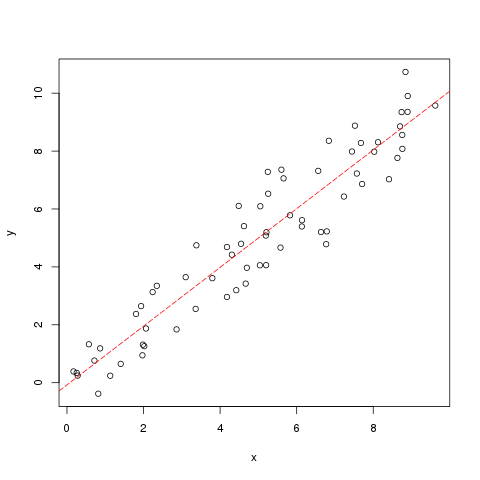
\includegraphics[scale=0.45]{a_regression/ordinary_least_squares_regression_result.png}
\caption{Plot 2D training dataset with the line of best fit.}
\label{plot:ordinary_least_squares_regression_result}
\end{figure}

% other packages ?


% References: Deeper understanding
% The references element description includes a listing of both primary sources of information about the technique as well as useful introductory sources for novices to gain a deeper understanding of the theory and application of the technique. The description consists of hand-selected reference material including books, peer reviewed conference papers, journal articles, and potentially websites. A bullet-pointed structure is suggested.
\subsection{References}
% What are the primary sources for a technique?
% What are the suggested reference sources for learning more about a technique?

% primary sources
\subsubsection{Primary Sources}
% least squares
The method for Least Squares may be traced back to Gauss who claims to have devised the method in and later published it in 1809 \cite{Gauss1809, Gauss1823} (Latin). Legendre independently developed and published the Least Squares method in 1805 \cite{Legendre1805} (Appendix, French).
% ordinary least squares specifically

% more info
\subsubsection{More Information}
% text books
Least Squares Regression is covered in any good text of statistics, data analysis or econometrics. Some popular introductory texts to least squares regression include Montgomery et~al.\ \cite{Montgomery2001} (Chapter 2), and Tamhane and Dunlop \cite{Tamhane2000} (Chapter 10).
% in R
Faraway provides a free book that includes a practical introduction into Least Squares Regression with examples in R \cite{Faraway2002} (updated version published \cite{Faraway2004}).


% END
\putbib\end{bibunit}
\newpage\begin{bibunit}% The Clever Algorithms Project: http://www.CleverAlgorithms.com
% (c) Copyright 2011 Jason Brownlee. Some Rights Reserved. 
% This work is licensed under a Creative Commons Attribution-Noncommercial-Share Alike 2.5 Australia License.

% Name
% The algorithm name defines the canonical name used to refer to the technique, in addition to common aliases, abbreviations, and acronyms. The name is used in terms of the heading and sub-headings of an algorithm description.
\section{Logistic Regression} 
\label{sec:logistic}
\index{Logistic Regression}
\index{logit}

% other names
% What is the canonical name and common aliases for a technique?
% What are the common abbreviations and acronyms for a technique?
\emph{Logistic Regression, Logit, Logit Model, Logistic Model, Binomial Logistic Regression, Binary Logistic Regression}

% Taxonomy: Lineage and locality
\subsection{Taxonomy}
% To what fields of study does a technique belong?
% What are the closely related approaches to a technique?
Logistic Regression is a regression method from the field of statistics, although us better understood as a classification method.
The most common form is Binomial Logistic Regression where the dependent variable is binary.
Logistic Regression may be considered a special case of Generalized Linear Regression.
Logistic Regression has many extensions including Ordered Logistic Regression that can handle ordinal dependent variables, and Multinomial Logistic Regression that can handle nominal (categorical) dependent variables.

What is Weighted Logistic Regression?
What is Stepwise Logistic Regression?
Where does Regularized Logistic Regression fit in?

% Strategy: Problem solving plan
% The strategy is an abstract description of the computational model. The strategy describes the information processing actions a technique shall take in order to achieve an objective. The strategy provides a logical separation between a computational realization (procedure) and a analogous system (metaphor). A given problem solving strategy may be realized as one of a number specific algorithms or problem solving systems. The strategy description is textual using information processing and algorithmic terminology.
\subsection{Strategy}
% What is the information processing objective of a technique?
Logistic Regression fits data to a logistic (sigmoidal) function and makes predictions of the probability of occurrence of an event. 
% What is a techniques plan of action?
A logistic function is used because it can take any values (positive or negative) and produce a value between 0 and 1. The logistic function is influenced by a logit function which take a variable derived from a sum of the weighted attributes. The logit function is the natural logarithm of the odds of the dependent variable equalling one.

The sign of a regression coefficient may be interpreted as the increase or decrease of an attribute to the resulting probability, and the magnitude represents the influence of the attribute.
The regression coefficients (weights) are fit by minimizing the maximum likelihood loss function. The problem as a system of linear equations use the Conjugate Gradient Method to solve the coefficients. Much research into the method is focused on more efficient algorithms for fitting the model.


% help me use this technique
\subsection{Overview}

% what it is good at
\subsubsection{Features}

\begin{itemize}
	\item Generally fast to create and results in an explainable model.
	\item Generally not parametrized, so there are no parameters to configure.
	\item Produces values always between zero and one. 
	\item Does not assume a linear relationship between the independent variables and the dependent variable. 
	\item Does not require normally distributed variables.
	\item The result is a probability of the occurrence of an event that may be interpreted as such and/or in turn be discretized to a binary classification prediction.
	\item More data can result in a better fit of the model.
	\item Training data with a minimum of 10 events per independent variable is recommended \cite{Peduzzi1996}.
	\item Features should be selected prior to fitting.
	\item Provides statistical test significance on a fitted model including: Wald Z-statistic, Likelihood-Ratio Test, and the Hosmer-Lemshow Goodness of Fit Test.
\end{itemize}

% what it is not good at
\subsubsection{Limitations}

\begin{itemize}
	\item The dependent variable must be binary (otherwise one must use another form of the method).
	\item The use of a logistic function means that input attributes can take any value, the bounds do not need to be known prior to building the model.
	\item It can only handle real-valued dependent variables.
	\item Dependent on the size of the sample used to prepare the model, smaller samples ($<1000$ or $<500$) can result in a model that overfits the training data.
	\item Solving the coefficients for large models can be very computationally expensive and remains an open area for research.
	\item Missing values must be handled explicitly or those records removed.
	\item Requires that the independent variable be related to the logit by a linear relationship.
\end{itemize}


% sample script in R
\subsection{Code Listing}
Listing~\ref{glm_logistic} provides a code listing of Logistic Regression in R using the \texttt{glm} (generalized linear model) function of the \texttt{stats} core package. 
% problem
The test problem is a contrived one dimensional problem where given a health statistic ($h$) determine whether a patient will survive or not $s\in\{0,1\}$.
The \texttt{gml} is distributed in core R and provides a number of functions besides the logistic function. By default, the method uses the Iteratively Re-weighted Least Squares (IWLS) method to fit.

% TODO make 2D problem and show the decision boundary + data points
% show stats?
% show convergence of gradient descent?

\lstinputlisting[firstline=7,language=r,caption={Example of Logistic Regression in R using the \texttt{glm} function of the \texttt{stats} core package.}, label=stats_logistic]{../src/algorithms/regression/stats_logistic_regression.R}

% References: Deeper understanding
% The references element description includes a listing of both primary sources of information about the technique as well as useful introductory sources for novices to gain a deeper understanding of the theory and application of the technique. The description consists of hand-selected reference material including books, peer reviewed conference papers, journal articles, and potentially websites. A bullet-pointed structure is suggested.
\subsection{References}
% What are the primary sources for a technique?
% What are the suggested reference sources for learning more about a technique?

% primary sources
\subsubsection{Primary Sources}

What are some primary sources for this method?

% more info
\subsubsection{More Information}
%Komarek and Moore provide promote the use of the method in modern data mining, suggesting modifications to the fit procedure to decrease computational complexity \cite{Komarek2005}.

There are many excellent books dedicated to Logistic Regression, some examples include 
``Logistic Regression: A Primer'' by Pampel that provides a practical introduction to the method \cite{Pampel2000}, ``Applied logistic regression'' by Hosmer and Lemeshow that provides a wealth of references \cite{Hosmer2000}, and ``Logistic Regression: A Self-Learning Text'' by Kleinbaum, Klein, and Pryor that is also an excellent self-paced introductory text \cite{Kleinbaum2010}.


% END\putbib\end{bibunit}
\newpage\begin{bibunit}% The Clever Algorithms Project: http://www.CleverAlgorithms.com
% (c) Copyright 2011 Jason Brownlee. Some Rights Reserved. 
% This work is licensed under a Creative Commons Attribution-Noncommercial-Share Alike 2.5 Australia License.

% Name
% The algorithm name defines the canonical name used to refer to the technique, in addition to common aliases, abbreviations, and acronyms. The name is used in terms of the heading and sub-headings of an algorithm description.
\section{Stepwise Regression} 
\label{sec:stepwise}
\index{Stepwise Regression}
\index{Stepwise Multiple Linear Regression}

% other names
% What is the canonical name and common aliases for a technique?
% What are the common abbreviations and acronyms for a technique?
\emph{Stepwise Regression, Stepwise Selection, Stepwise Multiple Linear Regression}

% Taxonomy: Lineage and locality
% The algorithm taxonomy defines where a techniques fits into the field, both the specific subfields of Computational Intelligence and Biologically Inspired Computation as well as the broader field of Artificial Intelligence. The taxonomy also provides a context for determining the relation- ships between algorithms. The taxonomy may be described in terms of a series of relationship statements or pictorially as a venn diagram or a graph with hierarchical structure.
\subsection{Taxonomy}
% To what fields of study does a technique belong?
Stepwise Regression is a Model Selection method for selecting a regression model. It was originally proposed as an extension to Multiple Linear Regression called Stepwise Multiple Linear Regression. It has since been generalized to other regression models, such as Logistic Regression for Stepwise Logistic Regression.

% What are the closely related approaches to a technique?
It is considered an improvement over Model Selection methods for Regression such as All Subsets, and is related to other Model Selection methods for Regression such as Ridge Regression. It is also related to Regularized Regression methods such as LASSO and the Least Angle Regression used to solve it.

% Strategy: Problem solving plan
% The strategy is an abstract description of the computational model. The strategy describes the information processing actions a technique shall take in order to achieve an objective. The strategy provides a logical separation between a computational realization (procedure) and a analogous system (metaphor). A given problem solving strategy may be realized as one of a number specific algorithms or problem solving systems. The strategy description is textual using information processing and algorithmic terminology.
\subsection{Strategy}
% What is the information processing objective of a technique?
The information processing objective of the technique is to result in a regression model that minimizes a specified measure, hypothesis test or criterion, for example F-tests in the original description, or more simply here as the minimum Sum Squared Residuals (SSR).
% What is a techniques plan of action?
A greedy hill-climbing algorithm that successively adds one of the remaining variables to the regression model that result in the largest reduction in the SSR and then refits the model. The procedure stops once no further improvements to the specified criterion can be achieved or there are no more variables to add to the model. This process alone is called Forward Model Selection. Conversely, the greedy algorithm may start with all variables and successively remove one that result in the largest decrease in the SSR. This approach alone is called Backward Selection.

Stepwise Regression applies Forward Model Selection as well as Backward Model Selection, allowing variables that have become redundant through the addition of other variables, to be removed from the model later in the process. This procedure requires the specification of threshold parameters for the minimum change in the of the selected measure for adding (F-to-enter) and removing (F-to-remove) variables to and from the model. The Forward method is applied until it can no longer add any more variables, then the Backward method is applied. This sequence repeats until the model stabilizes. One may start with no variables and successively grow a model, called Forward Stepwise Regression, or start with all variables and successively prune the model, called Backward Stepwise Regression.

% Heuristics: Usage guidelines
% The heuristics element describe the commonsense, best practice, and demonstrated rules for applying and configuring a parameterized algorithm. The heuristics relate to the technical details of the techniques procedure and data structures for general classes of application (neither specific implementations not specific problem instances). The heuristics are described textually, such as a series of guidelines in a bullet-point structure.
\subsection{Heuristics}
% What are the suggested configurations for a technique?
% What are the guidelines for the application of a technique to a problem instance?
\index{Akaike Information Criterion}
\index{AIC}
\index{Bayes Information Criterion}
\index{BIC}

\begin{itemize}
	\item Given the greedy nature of the selection procedure, neither Forward nor Backward Stepwise Regression generally result in the selection of an optimum model, but rather a sub-optimal model that is commonly close to the optimum model.
	\item It is typically applied to Linear Regression and Generalized Linear Regression Models.
	\item Modern implementations use hypothesis based tests to compare models (such as a t-test or an F-test) or criteria-based tests such as the Akaike Information Criterion (AIC) and the Bayes Information Criterion (BIC).
	\item Criterion tests for adding and removing variables such as AIC and BIC are preferred over hypothesis-based tests (such as the F-test) as the use of the latter have been discredited \cite{Pope1972, Wilkinson1979}.
	\item If the errors are normally distributed, the Akaike Information Criterion (AIC) selection criteria can be used \cite{Akaike1973}.
	\item Using a cross-validated error score for making decisions to add and remove variables may result in an improved final model.
	\item Resulting models frequently fail to include all variables that have an influence on the dependent variable while also frequently including variables that do not influence the dependent variable \cite{Derksen1992}, meaning the final model is generally not the best model \cite{Miller1984} (taken from \cite{Mundry2009}).
\end{itemize}

% sample script in R
\subsection{Code Listing}
% listing
Listing~\ref{stats_stepwise_linear_regression} provides a code listing of Stepwise Multiple Linear Regression method in R. Figure~\ref{plot:stepwise_regression_result} provides a plot of the training dataset with the line of best fit highlighted.

% algorithm and package
The example uses the \texttt{lm()} function and the and \texttt{step()} in the \texttt{stats} core package which are responsible for fitting linear models and performing stepwise selection respectively \cite{RDCT2011a}. The \texttt{step()} function uses a Akaike Information Criterion as the model evaluation criteria. For more information on this library type: \texttt{library(help="stats")}, and for more information on the function type: \texttt{?step}.

% problem
The test problem is a four-dimensional dataset of 100 samples, where the \texttt{x1}, \texttt{x2}, \texttt{x3} values are drawn from a uniformly random distribution $x \in [0,10]$ and \texttt{y} values are dependent on the \texttt{x1} value plus a value drawn from a normally random distribution with a mean of 0 and a standard deviation of 1. The features \texttt{x2} and \texttt{x3} are random independent variables that have no relevant interaction \texttt{x1} and \texttt{y}. In this example, \texttt{y} is considered the dependent variable and \texttt{x1} the single relevant independent. The stepwise method is expected to discount \texttt{x2} and \texttt{x3} and select a linear model for \texttt{y} given \texttt{x1}.

\lstinputlisting[firstline=7,language=r,caption={Example of Stepwise Multiple Linear Regression in R using the \texttt{lm()} and \texttt{step()} functions in the \texttt{stats} core package.}, label=stats_stepwise_linear_regression]{../src/algorithms/regression/stats_stepwise_linear_regression.R}

\begin{figure}[htp]
\centering
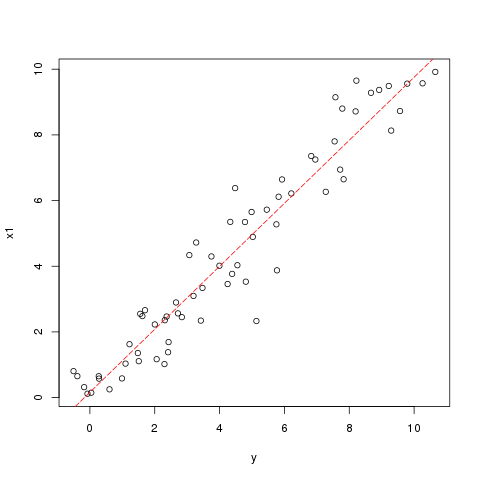
\includegraphics[scale=0.45]{a_regression/stepwise_regression_result.png}
\caption{Plot 2D training dataset with the line of best fit.}
\label{plot:stepwise_regression_result}
\end{figure}

% other packages
Other packages that provide stepwise selection include the \texttt{stepAIC()} function of the \texttt{MASS} package. The \texttt{leaps} package does not provide stepwise selection, although does provides a related selection method called Regression Subset Selection that uses a branch and bound search.

% References: Deeper understanding
% The references element description includes a listing of both primary sources of information about the technique as well as useful introductory sources for novices to gain a deeper understanding of the theory and application of the technique. The description consists of hand-selected reference material including books, peer reviewed conference papers, journal articles, and potentially websites. A bullet-pointed structure is suggested.
\subsection{References}
% What are the primary sources for a technique?
% What are the suggested reference sources for learning more about a technique?

% primary sources
\subsubsection{Primary Sources}
% seminal
Efroymson is credited with Stepwise Multiple Linear Regression in which he used an F-test significance for the add and remove decisions \cite{Efroymson1960}.
% early review
Breaux provides an early and salient overview of Efroymson's Stepwise Multiple Regression in his technical report that promotes the method as computationally efficient over enumerating all subsets of regression models \cite{Breaux1967}.

% more info
\subsubsection{More Information}
% general references
Hocking provides an early and detailed review of forward and backward variable selection methods and of Stepwise Multiple Linear Regression \cite{Hocking1976}.
Miller provides an analysis on the convergence of Stepwise Regression \cite{Miller1996}.
% stepwise is a bad idea
Whittingham et~al.\ provide a modern enumeration of all of the known problems and reasons against using Stepwise Multiple Regression for modelling, and fret about its commonplace use in the field ecology \cite{Whittingham2006}.
Mundry and Nunn provide a similar review and focus on the limitations of the method for statistical inference \cite{Mundry2009}.
% usage in R
Faraway provides a good example of stepwise procedures for regression with examples in R \cite{Faraway2002} (page 125).


% END
\putbib\end{bibunit}
\newpage\begin{bibunit}% The Clever Algorithms Project: http://www.CleverAlgorithms.com
% (c) Copyright 2011 Jason Brownlee. Some Rights Reserved. 
% This work is licensed under a Creative Commons Attribution-Noncommercial-Share Alike 2.5 Australia License.

% Name
% The algorithm name defines the canonical name used to refer to the technique, in addition to common aliases, abbreviations, and acronyms. The name is used in terms of the heading and sub-headings of an algorithm description.
\section{Multivariate Adaptive Regression Splines} 
\label{sec:mars}
\index{Multivariate Adaptive Regression Splines}
\index{MARS}
\index{MARSplines}
\index{Adaptive Regression Splines}

% other names
% What is the canonical name and common aliases for a technique?
% What are the common abbreviations and acronyms for a technique?
\emph{Multivariate Adaptive Regression Splines, MARS, MARSplines, Adaptive Regression Splines.}

% Taxonomy: Lineage and locality
% The algorithm taxonomy defines where a techniques fits into the field, both the specific subfields of Computational Intelligence and Biologically Inspired Computation as well as the broader field of Artificial Intelligence. The taxonomy also provides a context for determining the relation- ships between algorithms. The taxonomy may be described in terms of a series of relationship statements or pictorially as a venn diagram or a graph with hierarchical structure.
\subsection{Taxonomy}
% To what fields of study does a technique belong?
Multivariate Adaptive Regression Splines is a Multivariate Non-Parametric Regression method.
% What are the closely related approaches to a technique?
It is related to other Non-Parametric Regression methods such as Kernel Regression, Non-Parametric Multiplicative Regression, Additive Modelling and Regression Trees. The procedure to prepare the model is related to Regressive Partitioning for decision trees (CART). The use of forward and backward phases in regression shows some similarity to Stepwise Regression.
% extensions
Fast MARS in an extension of the canonical MARS method that suggests an optimization of the forward procedure when building the model.
% PolyMars?

% Strategy: Problem solving plan
% The strategy is an abstract description of the computational model. The strategy describes the information processing actions a technique shall take in order to achieve an objective. The strategy provides a logical separation between a computational realization (procedure) and a analogous system (metaphor). A given problem solving strategy may be realized as one of a number specific algorithms or problem solving systems. The strategy description is textual using information processing and algorithmic terminology.
\subsection{Strategy}
% What is the information processing objective of a technique?
The information processing objective of the technique is to find an equation that best describes the relationships between independent and a dependent variable.
% What is the model?
This is achieved by preparing a model that is the weighted sum of basis functions. A basis function can be as simple as a constant, or as complex as one or the product of multiple sub-functions that add non-linearities called hinge functions. Hinge functions take the form of $max(0, x-c)$ where $0$ is the minimum value for the function, $x$ is the variable, and $c$ is a constant (that provides a kink or sharp turn in one-dimension) called the knot. The number of basis functions as well as the parameters for each are determined determined automatically through an iterative process based on the data.

% what is the algorithm to arrive at the model?
MARS is motivated as a process to create a continuous model using a procedure like that used in recursive partitioning (CART). Like recursive partitioning, the method has a forward procedure to add terms and a backward procedure to prune terms from the model.
% forward
The forward procedure is a greedy algorithm that seeks to minimizes the sum of squared residual errors (SSR). It starts with the intercept and adds basis function terms to the model until a maximum number of terms have been added or no further improvements in SSR are possible. Terms are added and configured to give the greatest reduction in SSR.

% backward
The intent of the forward procedure is overfit the training data. The backward step is intended to add generality to the mode by pruning terms one-at-a-time selecting each term to remove based on the improvement in a generalized cross-validation score. The backward pass typically prunes one side of each pair of terms.
% cross validation score
The generalized cross-validation score is a performance measure that takes the complexity of the model and size of the training dataset as well as the SSR into account. The score seeks to minimize for model flexibility.

% Heuristics: Usage guidelines
% The heuristics element describe the commonsense, best practice, and demonstrated rules for applying and configuring a parameterized algorithm. The heuristics relate to the technical details of the techniques procedure and data structures for general classes of application (neither specific implementations not specific problem instances). The heuristics are described textually, such as a series of guidelines in a bullet-point structure.
\subsection{Heuristics}
% What are the suggested configurations for a technique?
% What are the guidelines for the application of a technique to a problem instance?

\begin{itemize}
	\item Friedman originally proposed it a suitable technique for sample sizes $50 \leq N \leq 1000$ and dimensions $3 \leq n \leq 20$.
	\item The algorithm requires the specification of the maximum number of terms to add in the forward pass. % recommended values?
	\item A penalty term (\texttt{d}) is used on the generalized cross-validation score which is commonly set to a small integer value ($d<4$, typically 2 or 3).
	\item Constraints can be imposed on the addition of terms in the first pass, such as limitations on the number of interactions permitted between basis functions. Low numbers of interactions are common (such as 1 or 2).
	\item It may be more suitable to real valued variables than recursive partitioning given the continuous nature of the hinge basis functions.
	\item Like partitioning, data preparation may not required as the hinge functions can account for outliers.
	\item The training times for MARS are relatively fast although it is a generally slower process than Recursive Partitioning on the same training dataset.
\end{itemize}

% sample script in R
\subsection{Code Listing}
% listing
Listing~\ref{earth_multivariate_adaptive_regression_splines} provides a code listing Multivariate Adaptive Regression Splines method in R to find a line of best fit for a two-dimensional data set.
% algorithm and package
The example uses the {earth()} function in the \texttt{earth} package that uses a generalized linear model as the underling method.
% problem
The test problem is a two-dimensional dataset of 50 samples, where the x-values are drawn from a uniformly random distribution $x \in [0,10]$ and y values are the x value plus a value drawn from a normally random distribution with a mean of 0 and a standard deviation of 1.

% code listing
\lstinputlisting[firstline=7,language=r,caption={Example of Multivariate Adaptive Regression Splines in R using the \texttt{earth} function of the \texttt{earth} package.}, label=earth_multivariate_adaptive_regression_splines]{../src/algorithms/regression/earth_multivariate_adaptive_regression_splines.R}

% other code examples
For more information on the \texttt{earth} package and function type \texttt{?earth}. Foulkes provides an example of using the \texttt{earth} package for genetic analysis \cite{Foulkes2009}. Mills provides an example using the \texttt{earth} package with sample output and plots of the model \cite{Mills2010}. Torgo also provides a small example if using the \texttt(earth) package \cite{Torgo2009}. 
% other package
Some other packages that provide an implementation of MARS include the \texttt{mda} package and the \texttt{polymars} package.


% References: Deeper understanding
% The references element description includes a listing of both primary sources of information about the technique as well as useful introductory sources for novices to gain a deeper understanding of the theory and application of the technique. The description consists of hand-selected reference material including books, peer reviewed conference papers, journal articles, and potentially websites. A bullet-pointed structure is suggested.
\subsection{References}
% What are the primary sources for a technique?
% What are the suggested reference sources for learning more about a technique?

% primary sources
\subsubsection{Primary Sources}
% seminal
MARS was proposed by Friedman in a paper that walks through the method in great detail and provides a number of case study datasets \cite{Friedman1991}.
% variable types
The approach was extended by Friedman to support both ordinal and categorical variables and missing values for this variable type \cite{Friedman1991a, Friedman1993a}.

% more info
\subsubsection{More Information}
% neural nets
The capability of representing non-linear relationships in the model using a number of basis functions likens the approach to artificial neural networks Friedman described the method in the context of neural networks, referring to it as `Adaptive Spline Networks' \cite{Friedman1991b, Friedman1991c}.
% Fast MARS
Friedman also suggested an improvement to optimize the forward pass procedure of the algorithm for large datasets called Fast MARS \cite{Friedman1993}.

% reviews
Friedman and Roosen provide an early introduction to the method with sample output from the FORTRAN program and clinical case studies \cite{Friedman1995}.
% R
Faraway provides a modern summary of the method and provides an example of using MARS using R \cite{Faraway2006} (page 271).


% END
\putbib\end{bibunit}
\newpage\begin{bibunit}% The Clever Algorithms Project: http://www.CleverAlgorithms.com
% (c) Copyright 2013 Jason Brownlee. Some Rights Reserved. 
% This work is licensed under a Creative Commons Attribution-Noncommercial-Share Alike 2.5 Australia License.


% Name
% The algorithm name defines the canonical name used to refer to the technique, in addition to common aliases, abbreviations, and acronyms. The name is used in terms of the heading and sub-headings of an algorithm description.
\section{Locally Estimated Scatterplot Smoothing} 
\label{sec:loess}
\index{Locally Weighted Regression}
\index{Locally Weighted Polynomial Regression}
\index{LOESS}
\index{LOWESS}
\index{Locally Estimated Scatterplot Smoothing}
\index{Locally Weighted Scatterplot Smoothing}

% other names
% What is the canonical name and common aliases for a technique?
% What are the common abbreviations and acronyms for a technique?
\emph{Locally Estimated Scatterplot Smoothing, LOESS, Locally Weighted Regression, LWR, Locally Weighted Polynomial Regression.}

% Taxonomy: Lineage and locality
% The algorithm taxonomy defines where a techniques fits into the field, both the specific subfields of Computational Intelligence and Biologically Inspired Computation as well as the broader field of Artificial Intelligence. The taxonomy also provides a context for determining the relation- ships between algorithms. The taxonomy may be described in terms of a series of relationship statements or pictorially as a venn diagram or a graph with hierarchical structure.
\subsection{Taxonomy}
% To what fields of study does a technique belong?
Locally Estimated Scatterplot Smoothing (LOESS) is a type of Local Regression and belongs to the general class of Non-Parametric Regression methods. It also belongs to the framework of Generalized Additive Models (GAMs).
% What are the closely related approaches to a technique?
LOESS is an extension to its precursor method Locally Weighted Scatterplot Smoothing (LOWESS).
It is related to other Non-Parametric Regression methods such as Multivariate Adaptive Regression Splines (MARS), Non-Parametric Multiplicative Regression, Additive Regression Model and Regression Trees. 

% Strategy: Problem solving plan
% The strategy is an abstract description of the computational model. The strategy describes the information processing actions a technique shall take in order to achieve an objective. The strategy provides a logical separation between a computational realization (procedure) and a analogous system (metaphor). A given problem solving strategy may be realized as one of a number specific algorithms or problem solving systems. The strategy description is textual using information processing and algorithmic terminology.
\subsection{Strategy}
% What is the information processing objective of a technique?
The information processing objective of the technique is to find an equation that best describes the relationships between independent and a dependent variable.
% What is a techniques plan of action?
This is achieved by fitting a local low-order polynomial model to nearby points, where `nearby' is defined by a distance kernel function (such as a nearest neighbor Euclidean distance kernel for continuous variables) between observations. A given polynomial model is fit using weighted least squares as needed,  where the response point is used as the centroid for the distance kernel function. The amount of data used to fit each local model is called the bandwidth or smoothing parameter. Regression models are created just-in-time for each response that is required.

% Heuristics: Usage guidelines
% The heuristics element describe the commonsense, best practice, and demonstrated rules for applying and configuring a parameterized algorithm. The heuristics relate to the technical details of the techniques procedure and data structures for general classes of application (neither specific implementations not specific problem instances). The heuristics are described textually, such as a series of guidelines in a bullet-point structure.
\subsection{Heuristics}
% What are the suggested configurations for a technique?
% What are the guidelines for the application of a technique to a problem instance?

\begin{itemize}
	\item LOESS is very simple, requiring only a sample of data to compute a local model for a given observation.
	\item The method delays computation until the time a response is needed, although computation at this time can be relatively demanding.
	\item The method is well suited to problems of time series prediction and two-dimensional data exploration (by projecting the line on a scatter plot of the data).
	\item It is common set the bandwidth parameter used to fit a local model using 25\% to 50\% of the given training dataset.
	\item It is common to use low order polynomials as local models, typically first (linear) or second (quadratic) degree. Higher order polynomials are expected to over-fit the data.
	\item It performs is as good as the training data, requiring relatively large non-sparse datasets (good local structure) to produce good predictions.
	\item It does not produce a single equation model like OLS that can be analyzed and understood.
\end{itemize}

% sample script in R
\subsection{Code Listing}
% listing
Listing~\ref{stats_locally_estimated_scatterplot_smoothing} provides a code listing of the Locally Estimated Scatterplot Smoothing method in R.
Figure~\ref{plot:locally_estimated_scatterplot_smoothing_result} provides a plot of the training dataset with the line of best fit highlighted.

% algorithm and package
The example uses the \texttt{loess()} function in the \texttt{stats} core package that provides Local Polynomial Regression Fitting using the LOESS method \cite{RDCT2011a}. For more information on this library type: \texttt{library(help="stats")}, and for more information on the function type: \texttt{?loess}.

% problem
The test problem is a two-dimensional dataset of 50 samples, where the \texttt{x}-values are drawn from a uniformly random distribution $x \in [0,10]$ and \texttt{y} values are the \texttt{x} value plus a value drawn from a normally random distribution with a mean of $0$ and a standard deviation of $1$.

% code listing
\lstinputlisting[firstline=7,language=r,caption={Example of Locally Estimated Scatterplot Smoothing in R using the \texttt{loess} function of the \texttt{stats} core package.}, label=stats_locally_estimated_scatterplot_smoothing]{../src/algorithms/regression/stats_locally_estimated_scatterplot_smoothing.R}

\begin{figure}[htp]
\centering
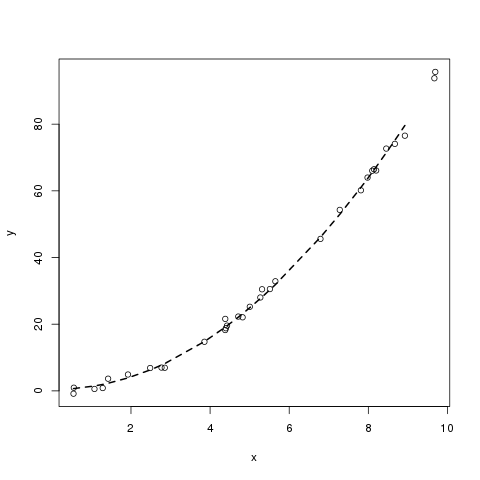
\includegraphics[scale=0.45]{a_regression/locally_estimated_scatterplot_smoothing_result.png}
\caption{Plot 2D showing the predicted line of best fit for the test dataset.}
\label{plot:locally_estimated_scatterplot_smoothing_result}
\end{figure}

% other packages
The \texttt{stats} package also provides an implementation of LOWESS in the \texttt{lowess()} function.

% References: Deeper understanding
% The references element description includes a listing of both primary sources of information about the technique as well as useful introductory sources for novices to gain a deeper understanding of the theory and application of the technique. The description consists of hand-selected reference material including books, peer reviewed conference papers, journal articles, and potentially websites. A bullet-pointed structure is suggested.
\subsection{References}
% What are the primary sources for a technique?
% What are the suggested reference sources for learning more about a technique?

% primary sources
\subsubsection{Primary Sources}
% precursor
Cleveland described a form of univariate local regression called Locally Weighted Scatterplot Smoothing (LOWESS) which also included a robust version of the method \cite{Cleveland1978, Cleveland1979}. 
This method was extended to the multivariate case by Devlin in an unpublished technical report \cite{Devlin1986}.
% seminal
Locally Estimated Scatterplot Smoothing (LOESS) or Multivariate Locally Weighted Regression is credited to Cleveland and Devlin \cite{Cleveland1988}.

% more info
\subsubsection{More Information}
% precursor
Cleveland presented a FORTRAN routine for LOWESS for data exploration \cite{Cleveland1981}.
% follow-ups
LOESS was further described by Cleveland et~al.\ \cite{Cleveland1988a}.
% implementation
LOESS was further developed by Cleveland and Grosse \cite{Cleveland1991} and later well described in terms of an implementation in S (Rs pre-cursor) \cite{Cleveland1992}.
% modern
Cleveland and Loader provide a more recent salient description of local regression including the history of the general method and examples \cite{Cleveland1996}.
Atkeson et~al.\ provide a broader survey of the field of locally weighted learning methods (lazy or memory-based learning), focusing on locally weighted linear regression \cite{Atkeson1997}.

% END
\putbib\end{bibunit}

